\section{Exponentialfunktionen}
Eine Exponentialfunktion stellt einen exponentiell Verlauf eines Graphen dar. 
\begin{figure}[h!]
\centering
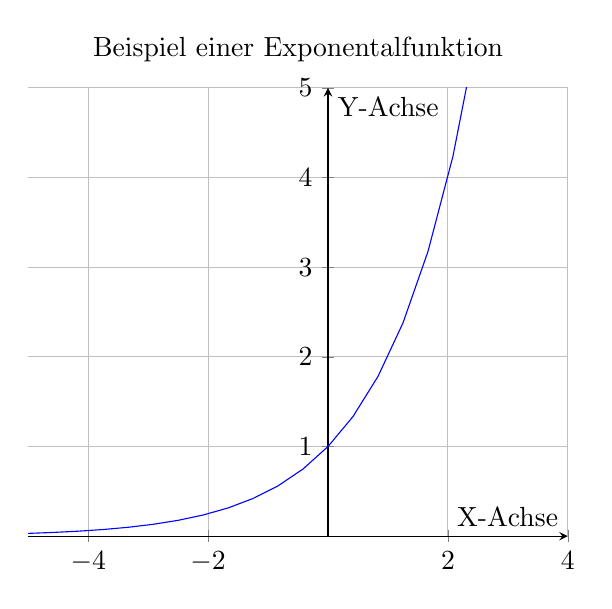
\begin{tikzpicture}
\begin{axis}[
    title={Beispiel einer Exponentalfunktion},
    xlabel={X-Achse},
    ylabel={Y-Achse},
    axis lines=middle, % Zentriert die Achsen
    xmin=-5, xmax=4, % Setzt die Grenzen für die X-Achse
    ymin=0, ymax=5, % Setzt die Grenzen für die Y-Achse
    grid=major, % Fügt ein Hauptgitter hinzu
]
% Hier fügen Sie Ihre Daten ein
\addplot+[mark=none] {2^x};
\end{axis}
\end{tikzpicture}
\caption{Funktionsgraph von $f(x)=2^x$}
\end{figure}

\subsection{Normalform}

Hierbei folgt einer Exponentialfunktion der folgenden Form: 
\[f(x)=a\cdot b^x\] Wobei $b>0 \land b\neq 0  $   sein muss.\\
 $a$ wird hierbei als Startwert bezeichnet. Innermathematisch spricht man von $a$ als Streckfaktor und von $b$ als Wachstumsfaktor. \\
 
 \subsubsection{Faktor \mbox{\boldmath$a$}  - Startwert} 
 Der Koeffizent $a$ stellt bei einer exponentiell verlaufenden Funktion den Startwert dar und zugleich auch Streckfaktor der Funktion. Er wird für jedes $x$ immer mit der Basis $b$ multipliziert. 
  \paragraph{Beispiel} sei sei $-0.5\le b\ge 2 $ und $-1\le a\ge 1$ für $f(x)=ab^x$
  \begin{align*} 
a&:-1			& a&:	0				&. a&: 1\\
x&:-1           &  x &: 0              &  x &:1\\
b&:-0.5			& b&:-0.5					& b&:-0.5\\
\\
f(-1)&=(-1)\cdot(-0.5)^{-1}	& f(0)&=0\cdot0.5^0	& f(1)&=1\cdot(-0.5)^1\\  
&= 2 & &=0 & &=-0.5\\
\end{align*}


  \subsubsection{Basis \mbox{\boldmath$b$} - Wachstumsfaktor } Die Basis $b$ ist hierbei von großer Bedeutung, da diese mit dem $x$ für jedes $x$ multipliziert wird. Da bei exponentiell Verläufen schnell das Vielfache der Basis erreicht wird, braucht der Wert von $b$ nur sehr gering sein, um eine große Auswirkung zu haben. Ebenfalls hat $b$ eine große Auswirkung den Verlauf in Bezug auf den Schnittpunkt mit der Y-Achse. $b$ ist hauptverantwortlich für diese, da durch $x$ die Anzahl der Multiplikationen mit sich selbst bestimmt wird. 


\paragraph{Beispiel} sei $-0.5\le b\ge 2 $ und $-1\le x\ge 2$ für $f(x)=b^x$
   	
\begin{align*} 
x&:-1           &  x &: 0              &  x &:1\\
b&:-0.5			& b&:-0.5					& b&:-0.5\\
f(-1)&=-0.5^{-1}	& f(0)&=a-0.5^0	& f(1)&=-0.5^1\\  
&= -2 & &=1 & &=-0.5
\end{align*}

\begin{align*}
x&:-1           &  x &: 0              &  x &:1\\
b&:0			& b&:0					& b&:0\\
f(-1)&=0^{-1}	& f(0)&=0^0	& f(1)&=0^1\\  
&= \infty & &=1 & &=0
\end{align*}

\begin{align*}
x&:-1           &  x &: 0              &  x &:1\\
b&:1			& b&:1					& b&:1\\
f(-1)&=1^{-1}	& f(0)&=1^0	& f(1)&=1^1\\  
&=1  & &=1 & &=1
\end{align*}

\begin{align*}
x&:-1           &  x &: 0              &  x &:1\\
b&:2			& b&:2					& b&:2\\
f(-1)&=2^{-1}	& f(0)&=2^0	& f(1)&=2^1\\  
&=0.5  & &=1 & &=2
\end{align*}
An dem Beispiel kann man sehen, dass egal welche Zahl die Basis $b$ annimmt es beim Einsetzten von
$0$ für $x$ immer zu $1$ kommt. Auffällig ist hierbei, dass setzt man für $b : 1$ ein, so erhält man zu jedem $x$ immer den Wert $1$. Dies ist die Begründung für die Schnittstelle mit der Y-Achse bei $1$, wenn $a=1$ ist. Setzt man nun für $b$ einen Wert ein, der größer als 1 ist, so verändert sich etwas. Die Basis $b$ wird für $x$ mit sich selber multipliziert. Nimmt $b$ nun einen Wert von $1.01$ an, so wird wie folgt für $x=3$ gerechnet. 
	\[\underbrace{1.01}_{1}\cdot\underbrace{1.01}_{2}\cdot\underbrace{1.01}_{3}\]
	\[=1.030301\]
	Die Differenz zwischen $1$ und $b$ wird vervielfacht. Alleine diese kleine Differenz reicht aus, um eine deutliche Ausprägung zu verursachen in dem Graphen von $f(x)$.
	
	
 
 %TODO Hier muss ein Beispiel kommen, warum sich b immer gleich auswirkt auf den Verlauf des Graphen. Auch ein Rechenbeispiel, welches zeigt, warum es dort eine Schnittstelle gibt und warum die prozentuale Steigung ensteht. 

 

 
 \subsection{Prozentuale Zunahme}
 Einen exponentiellen Verlauf kann man unteranderem an einer prozentualen Veränderung erkennen. So lässt sich sagen, dass sei $b>1$ eine prozentuale Steigung der Differenz zwischen
 $1$ und dem Wert, den $b$ annimmt bestimmen. \\
 Nimmt man an, dass sei $b=1.01$, so ist $0.1$ gleich $1\%$ von $1$ und besitzt somit eine prozentuale Zunahme von $1\%$. Übertragt man diesen Sachverhalt auf eine weitere Basis,
 welche $b>1$ erfüllt, so lässt sich ebenfalls der Übertrag als prozentuale Steigung definieren.
\paragraph{Beispiel} Sei \ $ b \in\{x : x \in \mathbb{R}, x > 1\}$ \
\[f(x)=1.04^x\Rightarrow4\%\]
So folgt aus $b=1.04$, dass eine Zunahme von $4\%$ vorliegt.\\
\\
\[f(x)=1.5^x\Rightarrow50\%\]
So folgt aus $b=1.5$, dass eine Zunahme von $50\%$ vorliegt.\\
\\
\[f(x)=1.9^x\Rightarrow90\%\]
So folgt aus $b=1.9$, dass eine Zunahme von $90\%$ vorliegt.\\
\\
\[f(x)=2.6^x\Rightarrow\ 160\%\]
So folgt aus $b=2.6$, dass eine Zunahme von $160\%$ vorliegt, da sich eine prozentuale Zunahme nur für die Differenz zwischen $b$ und $b=1$ ausprägt.\\
\\
\[f(x)=0.8^x\Rightarrow20\%\]
So folgt aus $b=0.8$, dass eine Abnahme von $20\%$ vorliegt. Zu dieser Annahme kommt man, indem man sich überlegt, dass $b=1=100\%$ sind. Hat man nun nur $b=0.8$ anstelle von $b=1$ , so ergibt sich hieraus die Verringerung von $20\%$
\pagebreak
\subsection{Prozentuale Zunahme/Abnahme algorithmisch bestimmen}
Um die Berechnung der prozentualen Änderung des Graphen zu bestimmen kann man algorythmisch vorgehen.
\begin{center}	
\tikzstyle{prozentuelleZunahme} = [rectangle, rounded corners, minimum width=3cm, minimum height=1cm, text centered, font=\normalsize, color=black, draw=f3551e38-74df-57e2-b793-83d7fe876c85, line width=1, fill=white]
\tikzstyle{Entscheidung} = [diamond, minimum width=3cm, minimum height=2cm, text centered, font=\normalsize, color=black, draw=f3551e38-74df-57e2-b793-83d7fe876c85, line width=1, fill=white]
\tikzstyle{Prozessbox} = [rectangle, minimum width=3cm, minimum height=1cm, text centered, font=\normalsize, color=black, draw=f3551e38-74df-57e2-b793-83d7fe876c85, line width=1, fill=white]
\tikzstyle{linie} = [thick, line width=1, ->, >=stealth]
\begin{tikzpicture}[node distance=2cm]
\node (ProzessBoxing) [prozentuelleZunahme] {Prozentuelle Zunahme};
\node (pfeil1) [Entscheidung, below of=ProzessBoxing, yshift=-0.5cm] {$b>1$};
\node (pfeil2) [Prozessbox, below of=pfeil1, yshift=-0.5cm,xshift=-3cm] {$b-1$};
\node (pfeil3) [Prozessbox, right of=pfeil2, xshift=4cm] {$1-b$};
\node (pfeil4) [Prozessbox, below of=pfeil2] {$\cdot100$};
\node (pfeil5) [Prozessbox, right of=pfeil4, xshift=4cm] {$\cdot100$};
\draw [linie] (ProzessBoxing) --  (pfeil1);
\draw [linie] (pfeil1) -| node[anchor=south] {ja} (pfeil2);
\draw [linie] (pfeil1) -| node[anchor=south] {nein} (pfeil3);
\draw [linie] (pfeil3) --  (pfeil5);
\draw [linie] (pfeil2) --  (pfeil4);
\end{tikzpicture}
\end{center}






